% !TEX root = _main.tex
% ========================================
% 制作環境：使ったソフト，手順（素材音はどこから，どうやって集めたか，出力方法等）
% ========================================

%1
\section{作品制作の環境と手法}
本章では，本研究における作品制作の環境と手法について整理する．

具体的には，作品制作に用いたソフトウェアやデータ形式，および音声素材の扱い方について述べる．

\subsection{作品制作の環境}
本節では，本研究における作品制作の環境について述べる．

具体的には，使用した DAW ソフトウェア，MIDI データを中心とした制作方法，およびサンプリングによる音声素材の利用について整理し，音のみを用いた物語作品を制作するための前提条件について解説する．

\vskip\baselineskip
\subsubsection{使用した DAW ソフトウェア}
本研究では，作品制作にあたり，DAW（Digital Audio Workstation）ソフトである Logic Pro  を使用した．

Logic Pro は，macOS 環境において標準的に利用可能なソフトであり，作品制作に必要なエフェクトや，音声素材を取り扱うためのサンプリング関連のプラグインがあらかじめ内蔵されている．

また，ピッチやベロシティの制御といった基本的な MIDI 編集機能を備えており，本研究で扱うような音による物語作品の制作に適している．

なお，本研究では Logic Pro を用いたが，同様に MIDI 編集機能とリバーブをはじめとしたエフェクト処理，および音声素材のサンプリングが可能な環境が整っていれば，他の DAW ソフトを用いても同種の作品制作は可能である．

\vskip\baselineskip
\subsubsection{MIDI データを中心とした制作方法}
本研究における作品は，主に MIDI（Musical Instrument Digital Interface）データを用いて制作している．

MIDI とは，音声そのものを記録する形式ではなく，音源を演奏する際のピッチ（音の高さ），ベロシティ（音の強さ），デュレーション（音の持続時間）などの演奏情報を記録したデジタルデータである．

この形式を用いることで，サンプリングした音声素材の演奏における各演奏情報を個別に操作することが可能となる．

一方で，雨や風といった環境音については，演奏情報の調整を行う必要がない場合も多いため，MIDI による制御を行わず，音声素材をオーディオデータとしてそのまま配置している．

本研究では，これらの MIDI パラメータを，登場キャラクターの鳴き声や身体動作，および出来事の推移を表現するための手段として用いている．

\vskip\baselineskip
\subsubsection{サンプリングによる音声素材の利用}
本研究では，作品制作にあたり，サンプリングの手法を用いている．

本研究におけるサンプリングとは，既存の音声素材を取り込み，編集や配置を行うことで，作品の構成要素として再利用する手法を指す．

本作品の制作においては，音声を新たに録音するのではなく，主にフリー音源配布サイトで提供されている音声素材を使用しており，これらを MIDI データまたはオーディオデータとして，音の役割に応じて使い分けながら構成している．

本研究における作品制作で利用したフリー音源配布サイトを，以下に示す．

\begin{enumerate}
  \item 効果音ラボ（https://soundeffect-lab.info/）
  \item Pixabay（https://pixabay.com/music/）
\end{enumerate}

\subsection{作品制作の手法}
本節では，本研究における作品制作の具体的な手法について述べる．

具体的には，物語作品をどのような単位で構成しているか，音声素材をどのように読み込むか，そしてそれらを用いてどのように表現上の工夫を行っているかについて述べる．なお，実際に作品中で行った具体的な工夫の内容については，次章において，個別のリージョンごとに詳しく述べる．

\vskip\baselineskip
\subsubsection{リージョンによる作品構成の整理}
本研究で対象とする物語作品は，連続した音の流れによって構成されているが，それは単一の音の連なりではなく，複数のイベントが連続することで物語として形成されている．このイベントに当たるのが，リージョンである．

リージョンとは，MIDI データやオーディオデータをブロックとしてまとめた音のまとまりであり，時間軸上に配置されることで，物語を構成する出来事の単位として扱うことができる（図1参照）．

\begin{figure}[htbp]
\begin{center}
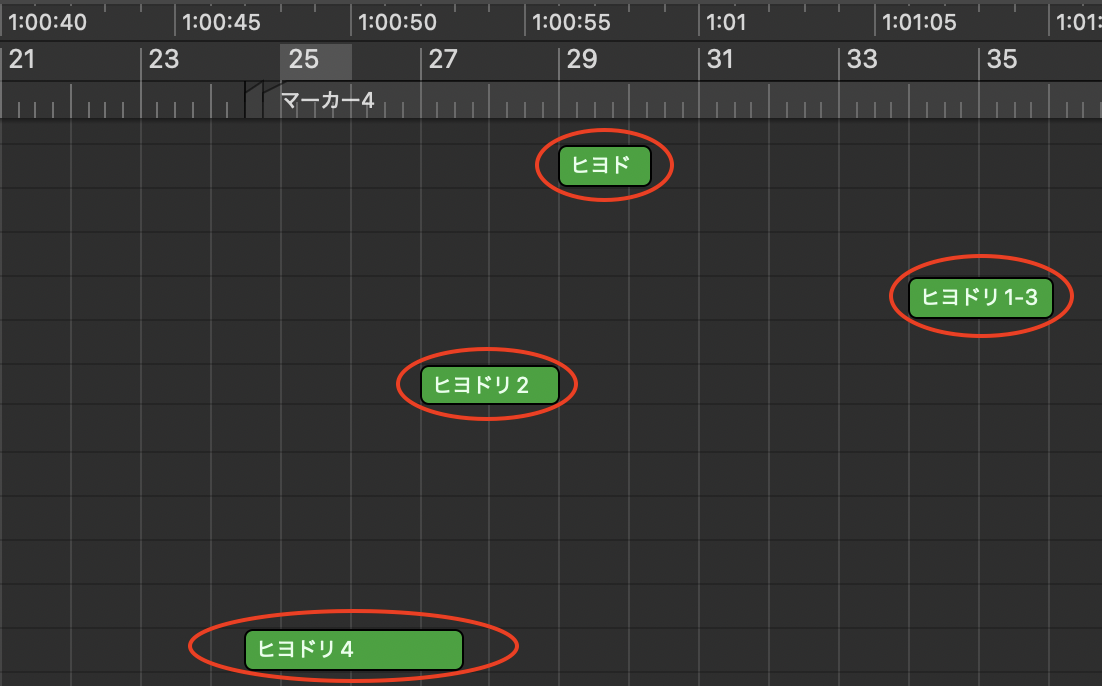
\includegraphics[width=70mm]{env1.png}
\caption{図1．DAW 上に配置されたリージョンの例（赤丸で囲った部分）}
\end{center}
\end{figure}

本研究では，リージョンを物語の構成単位として設定している．次小節以降では，リージョン内部において，音声素材をどのように用い，物語の具体的な出来事や展開を構成しているかについて述べる．

\vskip\baselineskip
\subsubsection{Quick Sampler の活用}
本研究における作品制作では，サンプリング機能を使用して各イベントの音声を作成するが，本小節では，サンプリングの手順について解説する．

各トラックで「Quick Sampler」を起動した後，音声素材のファイルをドラッグし，これをプラグインの画面上にドロップすることで，音声素材を読み込ませることができる（図2参照）．

\begin{figure}[htbp]
\begin{center}
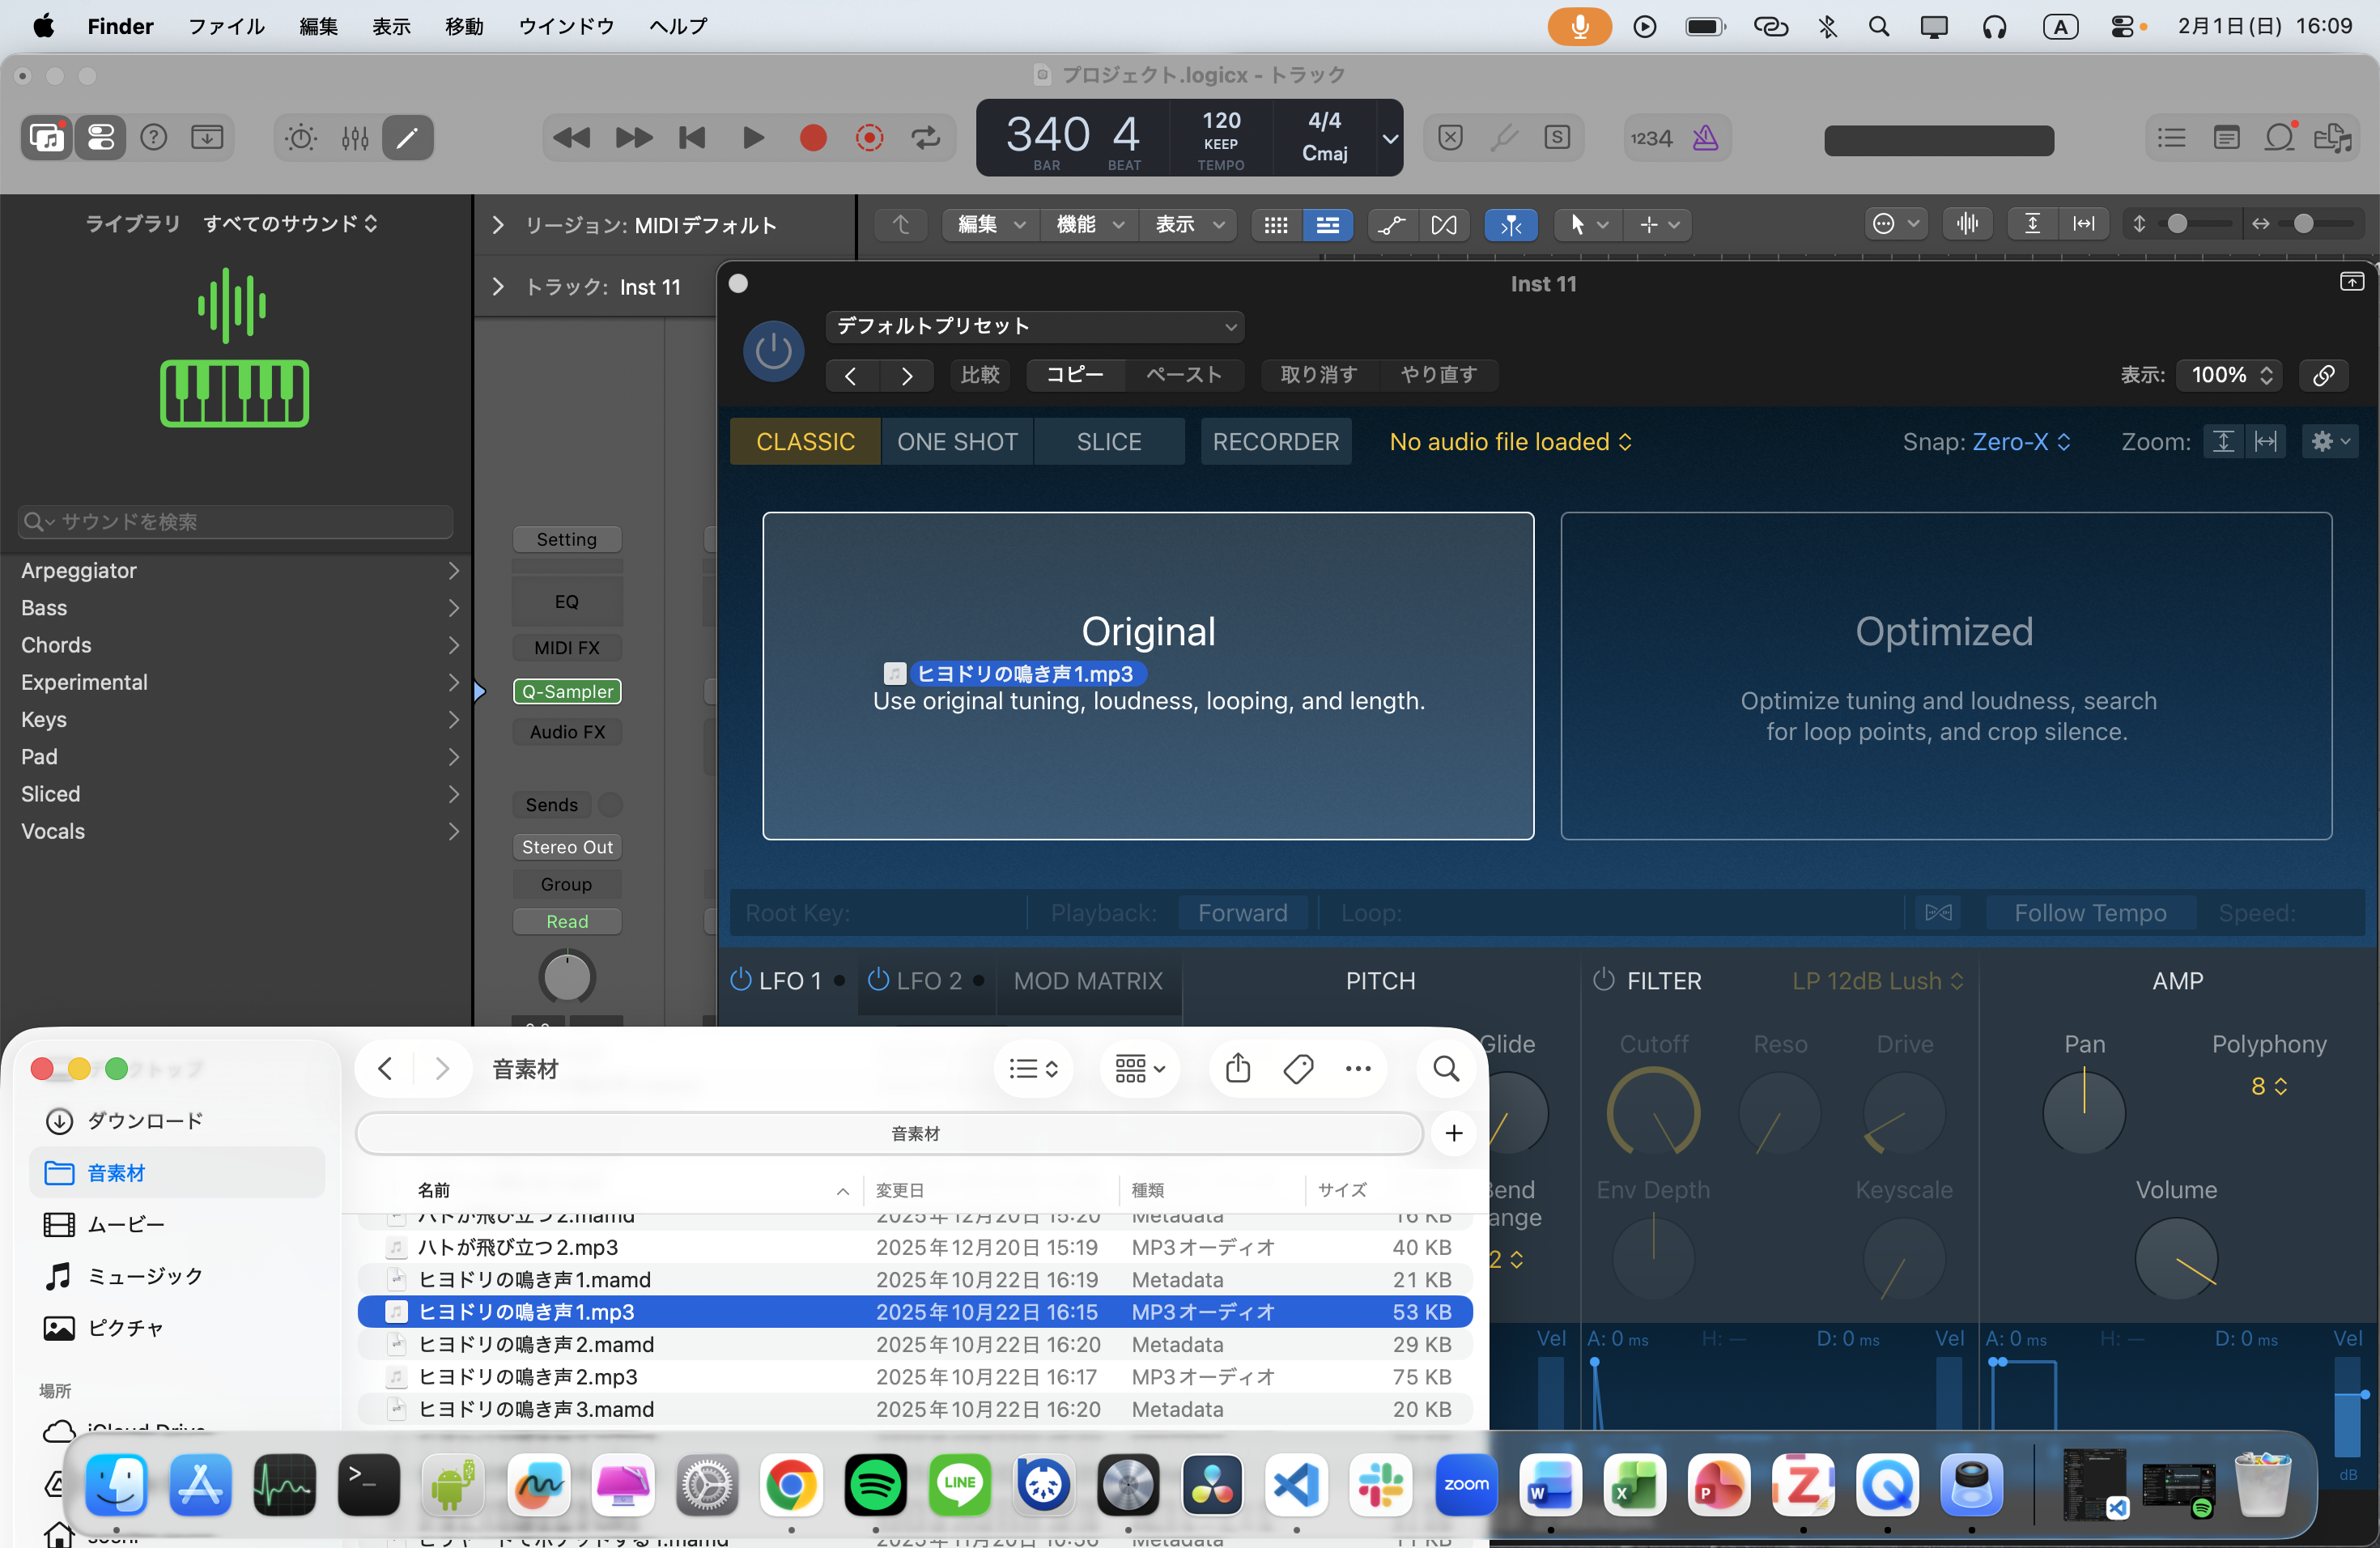
\includegraphics[width=70mm]{env2.png}
\caption{図2．Quick Samplerでの音声素材の読み込み}
\end{center}
\end{figure}

Quick Sampler では，音声素材の読み込み時に，もとのピッチや音量設定を保持する Original と，それらの最適化を自動的に行う Optimized を選択することができる．本研究では，音声素材の原音のピッチの基準を一貫して C3 として扱うため，音声素材の読み込みには Original を用いている．

音声素材のファイルを読み込むと，プラグインの画面にその音声素材の波形が表示される．この画面上では，音声素材のうち，MIDI データまたはオーディオデータとして再生に用いる部分を設定することができる（図3参照）．なお，Quick Sampler には，本研究で示したもの以外にもさまざまな機能が備わっているが，本研究では，作品制作に必要な基本的な機能に絞って使用している．

\begin{figure}[htbp]
\begin{center}
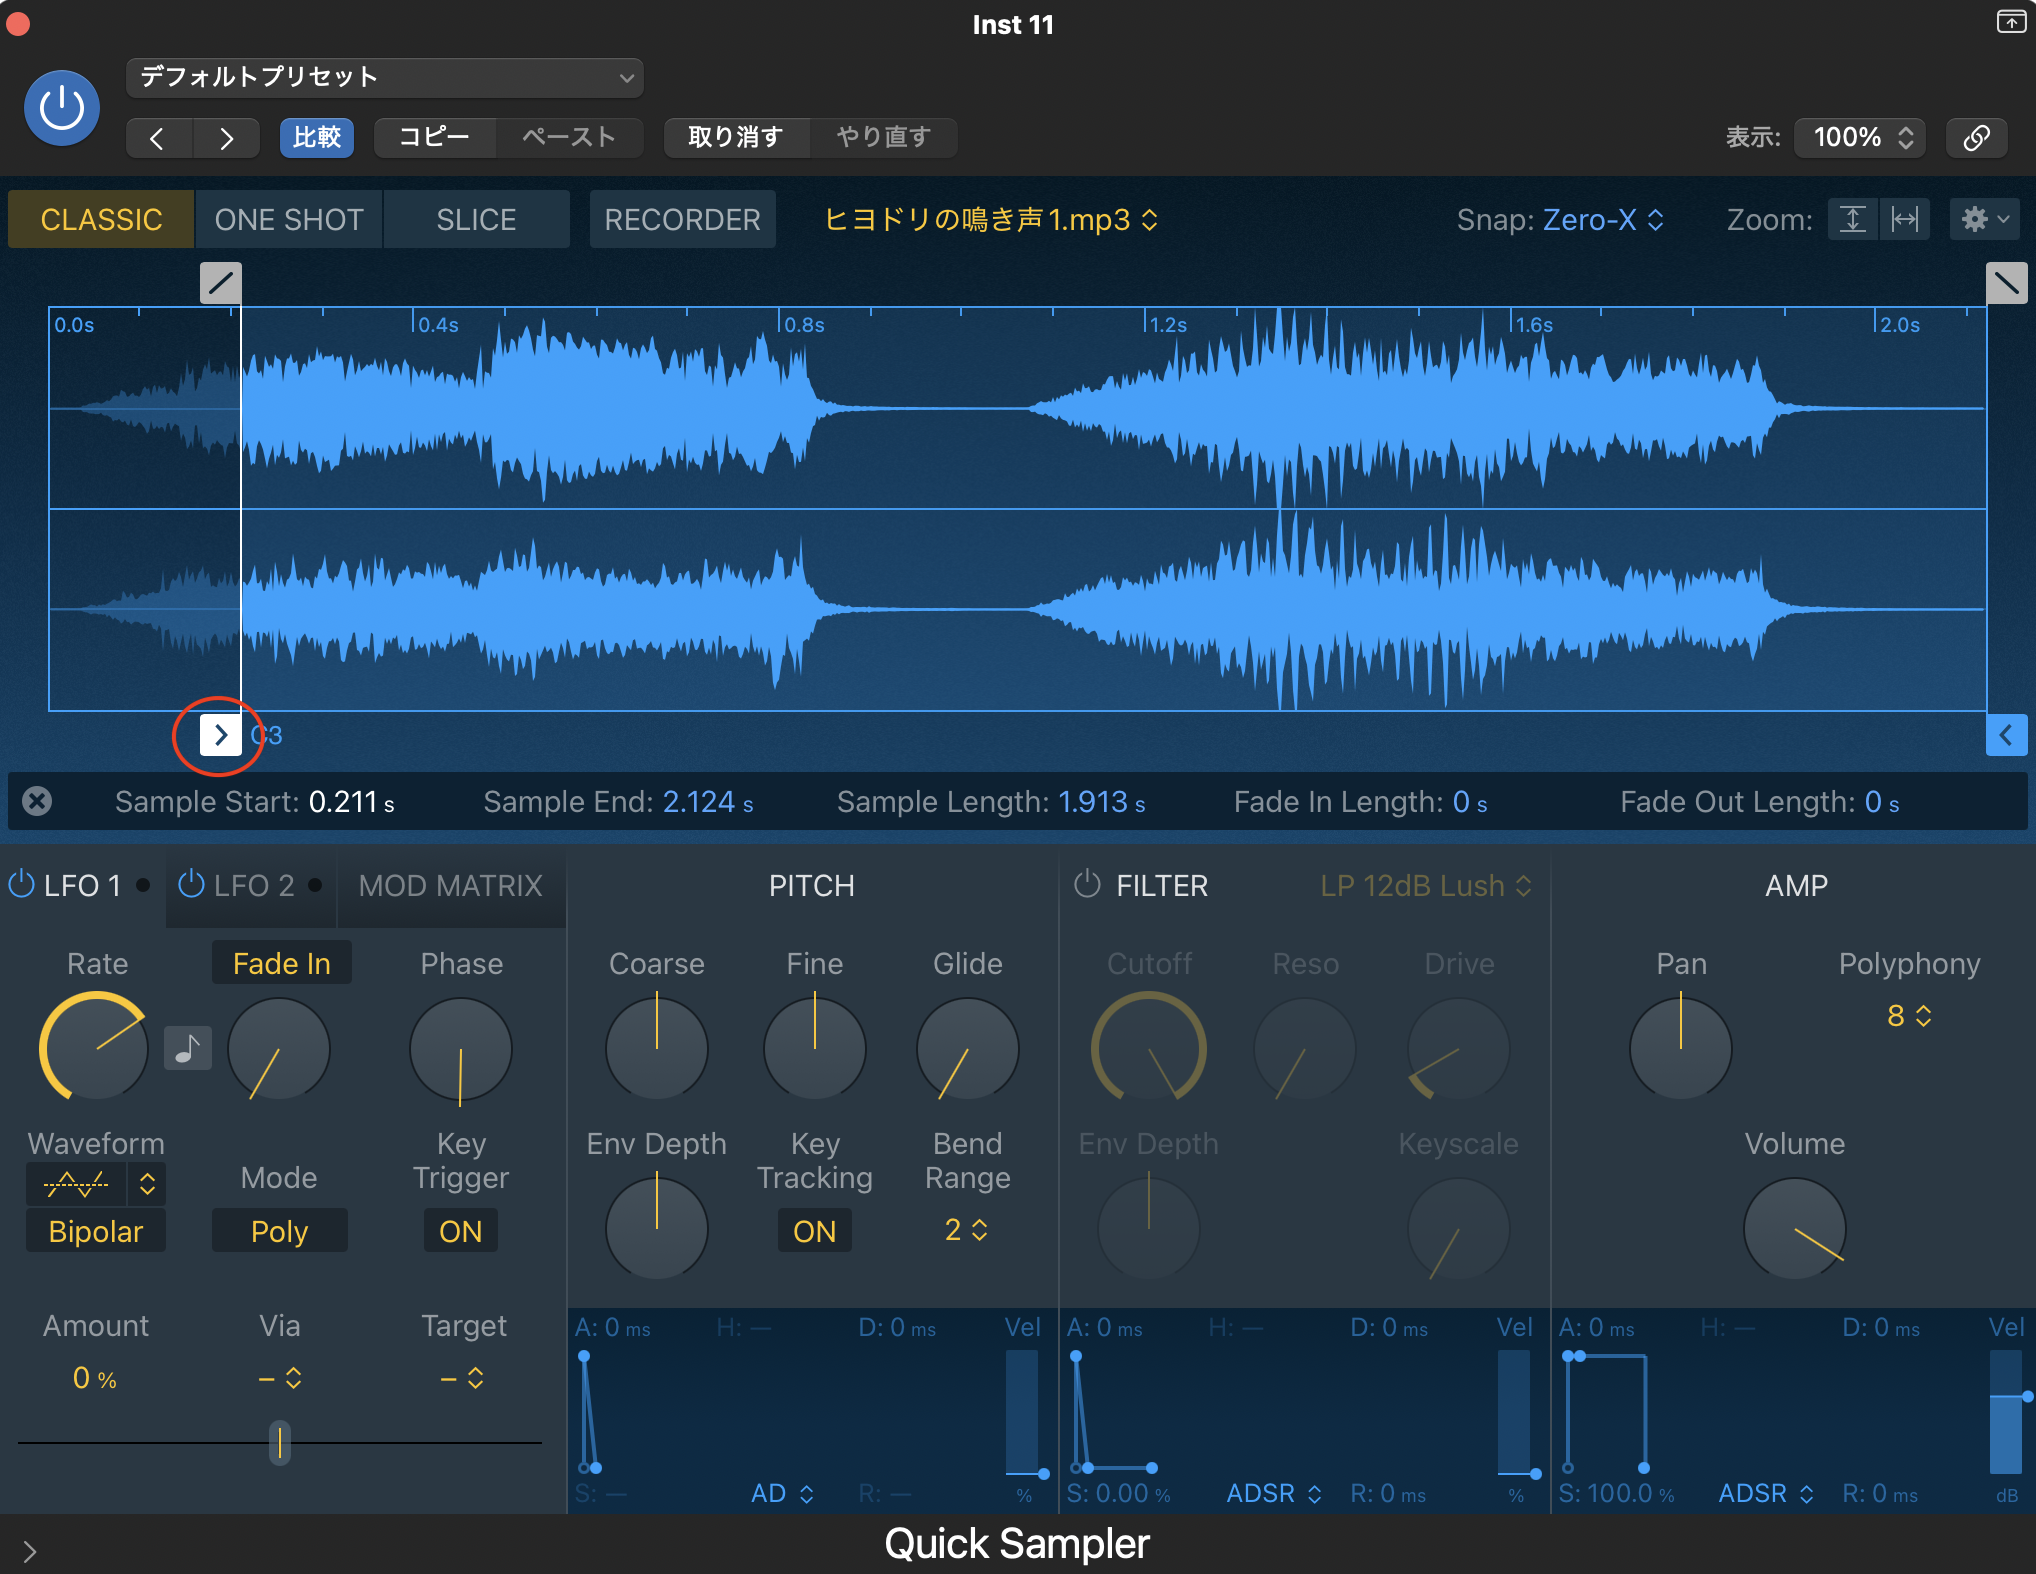
\includegraphics[width=70mm]{env3.png}
\caption{図3．音声素材の再生に用いる部分の設定（赤丸で示した操作部）}
\end{center}
\end{figure}

本小節では，Quick Sampler を用いたサンプリング機能の活用方法について述べた．次小節では，これらの音声素材を， MIDI データまたはオーディオデータとしてどのように扱い，作品内で活用しているかについて述べる．

\vskip\baselineskip
\subsubsection{MIDI データを中心とした音声素材の活用}
本研究では，サンプリングした音声素材を，MIDI データまたはオーディオデータとして配置している．登場キャラクターの鳴き声や効果音などを，ピッチやベロシティといった演奏情報の制御を通じて表現する場合には，音声素材を MIDI データとして扱っている．一方で，環境音を配置する場合など，演奏情報を個別に制御する必要のない音声素材については，オーディオデータとして配置している．なお，オーディオデータとして配置した音声素材についてもボリュームやエフェクトの設定は行っているが，本小節では，オーディオデータ特有の制御や編集方法について詳細に扱うことはせず，演奏情報の制御を通じた表現が可能な MIDI データを扱う際の工夫を中心に論じる．

以下では，演奏情報の制御を通じて物語内のイベントを能動的に表現する場面において，サンプリングした音声素材の活用方法について，心理的側面・物理的側面の2つの観点から，表現上の効果に着目して述べる．

物語の心理的な描写を表現する場面では，ピッチやタイミングの制御を通じて，態度の違いを聴覚的に示している．ピッチを高く設定することで，肯定的な反応として知覚されやすい場合がある一方で，場面によっては戸惑いや緊張を含んだ反応として受け取られることもある．逆に，ピッチを低く設定することで，落ち着きや警戒といった態度が示唆されやすい．また，音と音の間にわずかな時間を挟むことで，反射的ではない応答や，思考の過程を想起させる効果を持たせている．

物語の物理的な動作を描写する場面では，ベロシティやピッチといった演奏情報の制御に加え，ボリュームの調整やエフェクトの付与を通じて，動作の質や音響的な環境を聴覚的に示している．ベロシティの違いによって，登場キャラクターの動作の大きさや力強さの差を表現するとともに，ピッチの設定によって，動作の軽快さや重厚さの度合いを表現している．また，音声素材へのリバーブの付加やボリューム・ベロシティの調整によって，その登場キャラクターや現象との距離感を聴者に知覚させることができる．

\vskip\baselineskip
本章では，作品制作における環境および制作の手法について整理した．次章では，本章で示した制作環境と手法を前提として，実際に著者が作成した作品中のイベントを取り上げながら，音による物語制作がどのように行われているかについて，具体的な制作過程を通して述べる．
